\section{04.12.2024}{Wymiar homologiczny, $\asdim \Z^n=\asdim\R^n= n$}

Niech $X$ będzie zwartą przestrzenią metryczną. Definiujemy wówczas \buff{wymiar $\dim X$} jako najmniejsze $n$ takie, że dla każdego $\epsilon>0$ istnieje skończone pokrycie $U_\epsilon$ przestrzeni $X$ otwartymi zbiorami o średnicy $<\epsilon$ takie, że każdy $x\in X$ należy do $\leq (n+1)$ zbiorów z $U_\epsilon$.

\begin{example}
  $\dim([0,1]\times[0,1])\leq 2$
  Kwadrat możemy rozbić na dowolnie małe cegiełki średnicy $<\epsilon$
  \begin{center}
    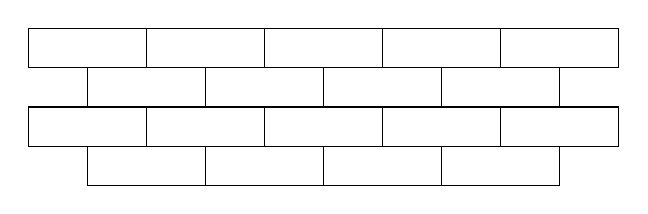
\begin{tikzpicture}
      \begin{scope}
        \draw (0,0)--(6, 0);
        \foreach \i in {0, 1.5, 3, ..., 6} \draw (\i, 0)--(\i, .5);
        \draw (-.75, .5)--(6.75, .5);
        \foreach \i in {-.75, .75, 2.25, ..., 6.75} \draw (\i, .5)--(\i, 1);
      \end{scope}
      \begin{scope}[shift={(0,1)}]
        \draw (0,0)--(6, 0);
        \foreach \i in {0, 1.5, 3, ..., 6} \draw (\i, 0)--(\i, .5);
        \draw (-.75, .5)--(6.75, .5);
        \foreach \i in {-.75, .75, 2.25, ..., 6.75} \draw (\i, .5)--(\i, 1);
      \end{scope}
      \draw (-.75, 1)--(0,1);
      \draw (6, 1)--(6.75,1);

      \draw (-.75, 2)--(6.75, 2);
    \end{tikzpicture}
  \end{center}
  i jako pokrycie wybrać malutkie otoczenia tych cegiełek. Wtedy każdy punkt jest w co najwyżej dwóch zbiorach.
\end{example}

\subsection{Wymiar asymptotyczny}

\begin{definition}{}{}
  Wymiar asymptotyczny $\asdim X$ to najmniejsze $n$ takie, że $(\forall\;R>0)$ istnieje (na ogół nieskończone) pokrycie $U_R$ przestrzeni $X$ zbiorami jednostajnie ograniczonymi (niekoniecznie otwartymi) takimi, że $(\forall x\in X)$ kula $B_R(x)$ należy do co najwyżej $(n+1)$ zbiorów z tego pokrycia.
\end{definition}

\begin{enumerate}
  \item $\asdim X$ jest niezmiennikiem q.i.
  \item $\asdim(\{n^3\;:\;n\in\Z\})=0$
  \item dla $X$ asymptotycznie spójnej, $\asdim X=0$ wtedy i tylko wtedy $X$ jest ograniczona
  \item $\asdim(\Z^n)\leq n$ (patrz: cegłówki wyżej)
  \item $\asdim (X\times Y)\leq \asdim (X)+\asdim(Y)$, ale łatwiej jest pokazać $\asdim(X\times Y)\leq \asdim X+\asdim Y+1$
  \item jeśli $Y\subseteq X$ z obciętą metryką, to $\asdim Y\leq \asdim X$
\end{enumerate}

Yu [1998] pokazał, że jeśli $\asdim G<\infty$, to $G$ spełnia hipotezę Novikova, a w 2003 Roe udowodnił, że $\asdim G<\infty$ $\implies$ $G$ zgrubnie zanurza się w przestrzeni Hilberta.

\begin{center}\slshape\large
Pytanie na dziś: jak pokazać, że $\asdim\Z^n=\asdim\R^n\geq n$?
\end{center}

\subsection{Dowód homologiczny}

Metoda homologiczna będzie polegała na:
\begin{enumerate}
  \item zdefiniowaniu $\asdim_h$ (asymptotyczny wymiar homologiczny)
  \item pokazaniu, że $\asdim_h\Z^n\geq n$
  \item na koniec wystarczy pokazać, że zwykły wymiar asymptotyczny jest nie mniejszy $\asdim \geq \asdim_h$.
\end{enumerate}

\begin{definition}{}{}
  Dla $\epsilon>0$ $q$-wymiarowy $\epsilon$-sympleks w przestrzeni metrycznej $X$ to układ $(x_0,x_1,...,x_q)$ punktów z $X$ (niekoniecznie różnych) takich, że $d_X(x_i, x_j)\leq\epsilon$ dla $0\leq i\neq j\leq q$.
\end{definition}

Określamy w oczywisty sposób $q$-wymiarowe $\epsilon$-łańcuchy, brzegowanie oraz $\epsilon$-homologie $H_q^\epsilon(X)$ [teoria homologii Alexandrowa].

Dla $\epsilon$-łańcucha $U$ w $X$ definiujemy nośnik $supp(U)$ jako zbiór wszystkich wierzchołków we wszystkich $\epsilon$-sympleksach z $U$ (mających niezerowy współczynnik).

Dla $\epsilon$-cyklu $z$, jego $\epsilon$-wypełnieniem nazywamy dowolny $\epsilon$-łańcuch $w$ taki, że $\partial w=z$.


%% OBRAZEK ZE JEST KWADRAT JAKO Z I JAK GO WYPELNIMY TROJKACIKAMI TO CALOSC JEST W TAKIE, ZE \PARTIAL W=Z
\begin{center}
  \begin{tikzpicture}
    \foreach \x in {0,..., 7} {
      \fill (\x, 0) circle (2pt);
      \fill (\x, 7) circle (2pt);
      \fill(0, \x) circle (2pt);
      \fill(7, \x) circle (2pt);
    }

  \end{tikzpicture}
\end{center}

\begin{definition}{}{}
  $\asdim_h(X)\leq p$ gdy dla każdego $\nu>0$ istnieje $\alpha>0$ (zależna tylko od $X$ i $\nu$) taka, że dla $q\geq p$ dowolny $q$-wymiarowy $\nu$-cykl $\phi$, $\nu$-homologicznie trywialny w $X$, jest także $\alpha$-homologicznie trywialny w swoim nośniku $supp(\phi)$.

  $\asdim_h(X)\geq n$ gdy istnieje $\nu$ takie, że dla każdego $\alpha$ istnieje $(n-1)$-wymiarowy $\nu$-cykl $\nu$-homologii $\phi$ trywialny w $X$ oraz $\alpha$-homologicznie nietrywialny w swoim nośniku.

  $\asdim_h(X)=\min \{p\;:\;\asdim_h(X)\leq p\}$
\end{definition}

Można pokazać, że $\asdim_h$ jest niezmiennikiem q.i..

% \subsection{Szkic dowodu, że $\asdim_h(\Z^n)=\asdmin_h(\R^n)\geq n$}


\begin{theorem}{}{}
  $$\asdim_h(\Z^n)=\asdim_h(\R^n)\geq n$$
\end{theorem}

{\large\color{red}TUTAJ ZDJECIA JAKIES CZY COS}

\begin{theorem}{}{}
  $$\asdim(X)\geq\asdim_h(X)$$
\end{theorem}





